\documentclass[10pt,a4paper]{article}
\usepackage[T1]{fontenc}
\usepackage[utf8]{inputenc}
\usepackage{lmodern}
\usepackage[margin=2.2cm]{geometry}
\usepackage{amsmath,amssymb}
\usepackage{graphicx}
\usepackage{booktabs}
\usepackage{tabularx}
\usepackage{xcolor}
\usepackage[colorlinks=true,linkcolor=blue!50!black,citecolor=blue!50!black,urlcolor=blue!50!black]{hyperref}
\usepackage{caption}
\captionsetup{font=small,labelfont=bf}
\usepackage{xspace}
\newcommand{\dBcm}{\,dB\,cm$^{-1}$\xspace}

\title{Laser-written photonic networks in silica under preregistered kill tests: mesh depth, crossings, in-situ calibration and energy limits}
\author{Francisco Angulo de Lafuente\\
\small Independent researcher \quad \url{https://github.com/Agnuxo1/Silice-Neuro3D-Cube}}
\date{13 October 2026 \quad (numerical study; no fabricated device)}

\begin{document}
\maketitle

\begin{abstract}
Three-dimensional waveguide networks written with femtosecond lasers inside glass are often presented as a route to compact, efficient optical linear layers and neural networks. We tested that promise for a silica-based project with four preregistered numerical and literature tests whose protocols, inputs and planned outputs were committed and verified on the hosting server before any result was computed. (i) Depth: three-dimensional connectivity can save at most one layer of a universal mesh of two-mode elements (bound $N-1$ for even $N$, $N$ for odd $N$; planar rectangular meshes need $N$). (ii) Crossings: a planar butterfly needs $\Theta(N^2)$ crossings (11 on the worst path at $N=16$ with free output order), but at the only verified crossing loss ($\le0.01$\,dB at 80$^\circ$) they cost about 0.1\,dB, less than the S-bends a three-dimensional route needs, so crossings alone do not decide. (iii) Energy: at $N=64$ and 8 bits the converters and modulators alone cost about 72\,fJ per multiply--accumulate, 1.4--4.5 times a 3\,nm INT8 digital macro, independently of the optical core; with the single published loss per fs-written interferometer stage, a dense passive layer needs 0.10\,nJ per MAC. The energy-advantage hypothesis fails its registered test. (iv) Calibration: in a model, in-situ recalibration brings the 95/95 bound of the infidelity of an 8-mode mesh with correlated 0.02\,rad splitter errors from $1.5\times10^{-2}$ to $1.3\times10^{-4}$. A verified literature review (31 records) places the state of the art for propagation loss at 1550\,nm at $0.06\pm0.02$\dBcm and shows precedents for three-dimensional fs-written Fourier circuits and neural networks. An independent adversarial review corrected the first wording of these claims. We therefore present a delimitation rather than a novelty claim, retain all negative results, name the measurements that would falsify it, and register the next physical test of the waveguide programme: a blind cut-back of trench waveguides whose ideal leakage floor (0.0020\dBcm at a 16\,\textmu m trench) is predicted in advance. No device was fabricated or measured.
\end{abstract}

\section{Introduction}

Femtosecond (fs) laser writing modifies the refractive index inside a glass volume and can draw waveguides, couplers and phase sections in three dimensions. It is therefore an attractive route to optical linear transforms, and to the linear layers of optical neural networks, written inside a monolithic block of silica. The idea is not new: programmable interferometers \cite{Kondratyev2024,Pentangelo2024} and a multilayer three-dimensional photonic neural network \cite{Cao2026} have already been written with fs lasers in glass. This study asks a narrower question: \emph{which advantages of a three-dimensional, laser-written network in silica survive quantitative tests that could have failed, before any device is fabricated?}

The project behind this paper (Silice-Neuro3D-Cube) produced numerical models of trench (depressed-cladding) waveguides at 1550\,nm, a set of retained negative results and a graphics-pipeline experiment. Its earlier claims were partly superseded by the literature. We therefore (i) froze an integrity framework (git-anchored preregistration verified on the hosting server, blind-analysis tools, a claims ledger and a three-zone decision rule), (ii) ran four preregistered tests designed to kill candidate headline claims, and (iii) chose a single central claim with a decisive physical test. All results here are numerical models or literature syntheses. None is a measurement.

\section{Integrity framework}

\paragraph{Preregistration anchored in git and on the server.} Each test has a JSON protocol with model, units, acceptance criteria, decision rule and the list of planned artifacts. The protocol and its sources are committed and pushed; a commitment record stores the commit, the git blob identifiers and a server check (\texttt{git ls-remote}) that the commit is published. The audit re-reads the protocol from the committed object (not from a copy that could be edited), rejects changed sources, artifacts that pre-date the commitment or were never planned, and other committed versions of the same protocol. A residual limit remains: a protocol committed for the first time after the data were produced is not detectable from the repository alone.

\paragraph{Amendments and failures.} One run (T25) crashed while writing its results. The crash was kept, its partial outputs were archived unopened, and a dated amendment with a new identifier was committed and published before the rerun. Failed executions cannot pass the audit by construction.

\paragraph{Claims ledger and decision rule.} Every public statement comes from a ledger whose entries carry a scope, a status, a falsifier and hashed evidence of the kind the scope requires (a simulation never closes a physical claim; agreement between the project's AI agents never counts as replication). Interval decisions use a three-zone rule: CONFIRMED if the upper bound of the 95\,\% interval is below the threshold and the lower bound is above the model floor; FALSIFIED if the lower bound exceeds the threshold; MODEL\_CONTROL\_FAIL if the whole interval lies below an ideal model floor; INCONCLUSIVE otherwise.

\paragraph{Software.} The tools (\texttt{agentkit}) pass 61 tests on Windows and Linux in a hash-locked environment, and continuous integration checks that the committed code is byte-identical to the specification document.

\section{Models carried over from earlier work}

Table~\ref{tab:prior} summarizes the earlier numerical results that the kill tests build on, with their registered status. The waveguide is a trench (depressed-cladding) guide with core index $n_0=1.444$ (consistent with the SK-1310 datasheet, which follows Malitson's fused-silica dispersion offset by $+6\times10^{-4}$), trench contrast $\Delta n=-0.005$, core radius $a=6$\,\textmu m and trench width $t=12$\,\textmu m, at $\lambda=1550$\,nm.

\begin{table}[h]
\centering\small
\begin{tabularx}{\linewidth}{>{\raggedright\arraybackslash}p{3.6cm}X>{\raggedright\arraybackslash}p{2.6cm}}
\toprule
Item & Result & Status \\
\midrule
Vector leakage of the trench guide & HE$_{11}$: $n_\mathrm{eff}=1.442189$, leakage 0.044\dBcm; TE$_{01}$/TM$_{01}$: 2.75--2.79\dBcm & model (layer solver) \\
Scalar versus vector & TE/TM splitting $\sim3\times10^{-6}$; scalar finite differences reach $4.2\times10^{-6}$ at $h=0.125$\,\textmu m (order 1.4) and cannot resolve it & partial (T06) \\
Paraxial BPM loss artefact & guided-mode loss $2.8\times10^{-8}$ and $2.7\times10^{-8}$\,mm$^{-1}$ at $\Delta z=0.125$ and 0.0625\,\textmu m; artefact for $\Delta z\ge0.25$\,\textmu m & partial \\
Time convergence of the D16 model & two audits passed; the fine run F1 stopped at 96/192 fields and its outputs were not recovered & open (T01) \\
Calibration-aware compiler & C1 met; C2 failed ($1.3$--$1.7\times10^{-2}$ vs $5\times10^{-3}$); C3 met in 28/36 realizations (77.8\,\%, exact 95\,\% CI 60.8--89.9\,\%) & partial (T11) \\
Correlated phase errors & H10b failed: a correlation length raised the 95th percentile by a factor 1.68 (registered band 0.8--1.25) & partial (T10) \\
Small optoelectronic network F3-b & 64.25\,\% test accuracy vs 84.55\,\% for a non-converged electronic reference; majority class 52.5\,\% & registered negative (T12) \\
Graphics-pipeline field rendering & R1, R2, P1 failed precision; R3 rendered 84/84 analytic fields per backend within $5.9\times10^{-7}$ (representation only, not propagation) & mixed \\
\bottomrule
\end{tabularx}
\caption{Earlier numerical results and their registered status (details and hashes in the claims ledger).}
\label{tab:prior}
\end{table}


\section{Kill tests}

\subsection{T25: depth and crossings of planar and three-dimensional meshes}

\emph{Question.} Can writing in three dimensions reduce the depth, crossings or error accumulation of a photonic mesh? \emph{Registered criteria} were seven computational consistency checks; all were met. Figure~\ref{fig:t25} shows the results.

\paragraph{Depth.} The real dimension of $U(N)$ is $N^2$. A general two-mode element is a $U(2)$ with four parameters, but common-mode phases commute through the mesh and collect in one output phase screen of $N$ phases, so each element adds at most two independent parameters. With $\lfloor N/2\rfloor$ disjoint elements per layer, a mesh of depth $D$ has at most $N(D+1)$ parameters for even $N$, so universality needs $D\ge N-1$ for even $N$ and $D\ge N$ for odd $N$, whatever the connectivity. Measured on random unitaries for $N=3$--16, the rectangular (Clements) synthesis \cite{Clements2016} has depth $N$ and the triangular synthesis $2N-3$ (reconstruction error $\le3.8\times10^{-15}$). A cylindrical arrangement, in which the first and last modes also couple (natural only in three dimensions), reaches full local Jacobian rank at depth $N-1$ for $N=4$, 6 and 8 (review scripts), although its global universality was not tested. \textbf{Three-dimensional connectivity can save at most one layer.}

\paragraph{Crossings.} A radix-2 butterfly realizes the unitary DFT with $(N/2)\log_2N$ couplers in $\log_2N$ stages (factorization error $2.2\times10^{-14}$). In an explicit planar layout, adjacent swaps bring partners together and back; the total number of crossings is $N(N-1-\log_2N)/2$, and the worst light path crosses 2, 7, 18, 41 and 88 guides for $N=4$, 8, 16, 32 and 64 (dynamic programme checked against brute force for $N\le32$). This layout is optimal within its family for fixed input and output order; freeing the output order, which a DFT allows, halves the total and gives worst paths of 4, 11, 26 and 57 crossings for $N=8$, 16, 32 and 64. Any planar layout still needs $\Theta(N^2)$ crossings. A three-dimensional butterfly needs no crossings but needs transitions between planes. Its crossing advantage is measurable only if the loss per crossing exceeds $2U/X(N)$, where $X(N)$ is the worst-path count and $U=0.2$\,dB is an assumed repeatability of an insertion-loss difference: 0.022\,dB per crossing at $N=16$ with fixed order, 0.036\,dB with free output order.

\paragraph{Errors.} With splitter-angle errors of 0.02\,rad, the butterfly DFT (32 couplers at $N=16$) keeps a 5th-percentile fidelity of 0.9989, against 0.9923 for the Clements DFT (240 couplers); a shared error component widens the tail of both. The butterfly is not universal, so this compares different function classes and applies only to tasks that need a structured transform.

\begin{figure}[t]
\centering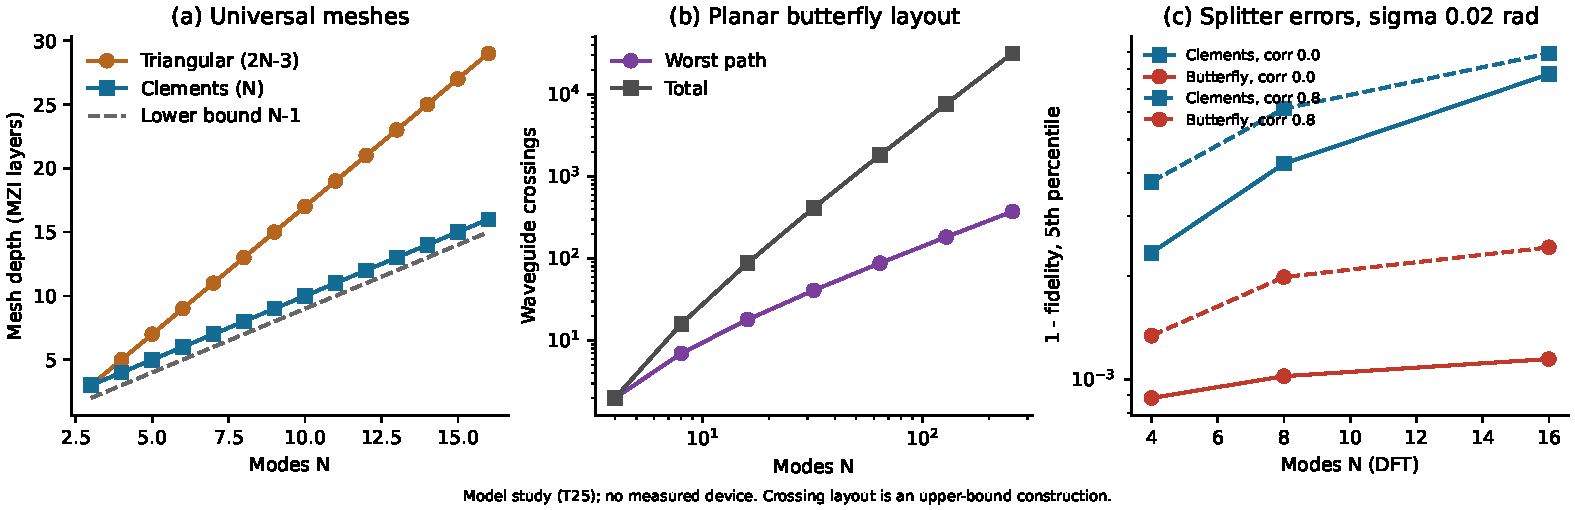
\includegraphics[width=\linewidth]{figures/fig_t25_scaling.pdf}
\caption{T25 (model). (a) Depth of universal meshes against the bound $N-1$. (b) Crossings of the planar butterfly layout. (c) 5th-percentile infidelity of the DFT under splitter errors, Clements versus butterfly.}
\label{fig:t25}
\end{figure}


\subsection{T27: in-situ recalibration of fabrication errors}

\emph{Question.} Fs-written couplers have fabrication errors, partly shared across a chip. Can in-situ recalibration of a programmable mesh absorb them? \emph{Registered criteria} at the primary point ($N=8$, $\sigma=0.02$\,rad, 80\,\% of the variance shared, 60 Haar-random targets): the distribution-free 95/95 upper bound of the infidelity after calibration $\le10^{-3}$, and a median improvement $\ge10$. Both were met (Fig.~\ref{fig:t27}).

Programming the ideal phases leaves a median infidelity of $1.6\times10^{-3}$ and a 95/95 bound of $1.5\times10^{-2}$. Re-optimizing every phase on the erroneous device with an exact analytic gradient brings the median to machine precision and the 95/95 bound to $1.3\times10^{-4}$; five of 60 targets remain unreachable, between $5\times10^{-6}$ and $1.3\times10^{-4}$. An 8-bit phase DAC sets a floor of about $2\times10^{-4}$. Precompensation on a model whose splitter errors are characterized to $0.1\sigma$ reaches a 95/95 bound of $1.6\times10^{-4}$. At $\sigma=0.05$\,rad with independent errors the $10^{-3}$ level is not reached ($2.3\times10^{-3}$). The model omits thermal crosstalk, drift, loss and measurement noise, and assumes exact access to the device transfer matrix.

\begin{figure}[t]
\centering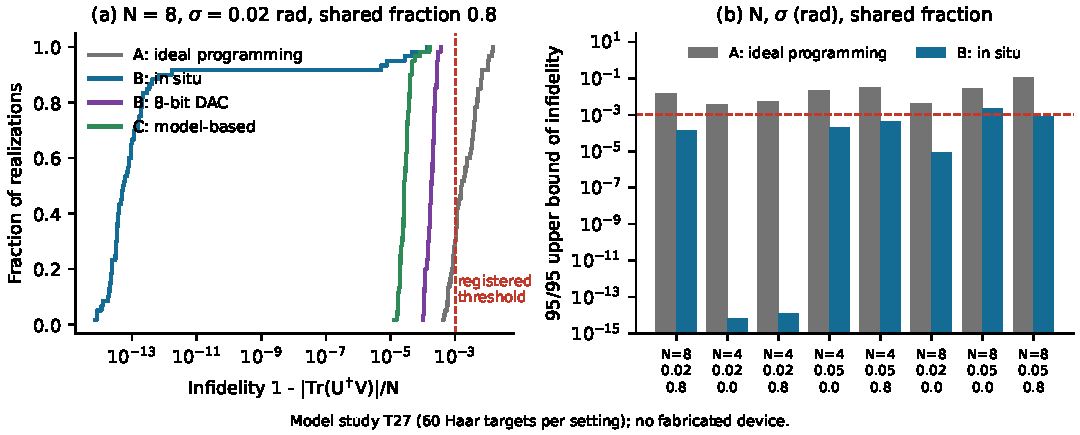
\includegraphics[width=\linewidth]{figures/fig_t27_calibration.pdf}
\caption{T27 (model). (a) Distribution of the infidelity at the primary point for ideal programming, in-situ calibration, 8-bit quantization and model-based precompensation. (b) 95/95 upper bounds before and after calibration across the secondary grid; the dashed line is the registered threshold.}
\label{fig:t27}
\end{figure}


\subsection{T24: energy per multiply--accumulate}

\emph{Question.} Could a passive optical layer in silica, with all its electronics, need less energy per multiply--accumulate (MAC) than a digital reference at equal 8-bit precision? The protocol fixed the primary point (dense $64\times64$ layer, 8 bits, 1\,GS/s), the parameter-selection rules (nominal: typical cited value; optimistic: best demonstrated value), two digital references and the decision rule before any value was gathered. Component values were then collected and identifier-checked (22 DOIs), frozen and published, and only then was the budget computed with a shot- plus thermal-noise detector model \cite{Hamerly2019,McMahon2023}.

The optimistic budget is 0.10\,nJ per MAC, against 0.23\,pJ for 8-bit arithmetic at 45\,nm \cite{Horowitz2014} and 0.016\,pJ for a 3\,nm INT8 digital compute-in-memory macro (124.6\,TOPS/W at 0.5\,V). The advantage factors are $2.3\times10^{-3}$ and $1.6\times10^{-4}$; the nominal set is a further order of magnitude worse. The registered criterion fails. The robust part of this verdict does not depend on the optics: at $N=64$ the converters and modulators alone cost 71.6\,fJ per MAC with the optimistic values, 4.5 times the 3\,nm macro at 0.5\,V and about 1.4 times at nominal voltage, so the comparison with modern digital hardware is lost even for a lossless optical core. The size of the gap depends on the mesh, and three choices made after the commitment (all against the hypothesis) set it: the SVD realization, the single published stage loss for fs-written interferometers (0.35\,dB, measured in borosilicate) used in both sets, and single-mode laser values. The optimistic set is, conversely, lenient on electronics ($k=1$ at half an LSB, a binary modulator energy, an ADC of effective resolution 7.3 bits, no static power). With these choices: a general passive layer realized by singular-value decomposition needs two universal meshes, $2N=128$ MZI layers at 0.35\,dB each \cite{Ceccarelli2020}, about 45\,dB, which multiplies the laser energy by $\sim3\times10^4$ and exceeds the 22 (nominal) or 77 (optimistic) stages the laser power can feed. An exploratory variant with a lossless mesh still loses at $N=64$ (advantage 0.21). Break-even with the modern reference would need $N\approx300$ even without mesh loss (Fig.~\ref{fig:t24}). Against the 2014 reference the verdict is fragile: a stage loss of at most 0.13\,dB would reverse it, and 0.07\,dB per stage gives 98\,fJ per MAC, 2.3 times better than the 45\,nm MAC. Programmable glass meshes add heater power: 4032 thermo-optic shifters at 31.5\,mW mean draw 127\,W in air \cite{Pentangelo2024}.

\begin{figure}[t]
\centering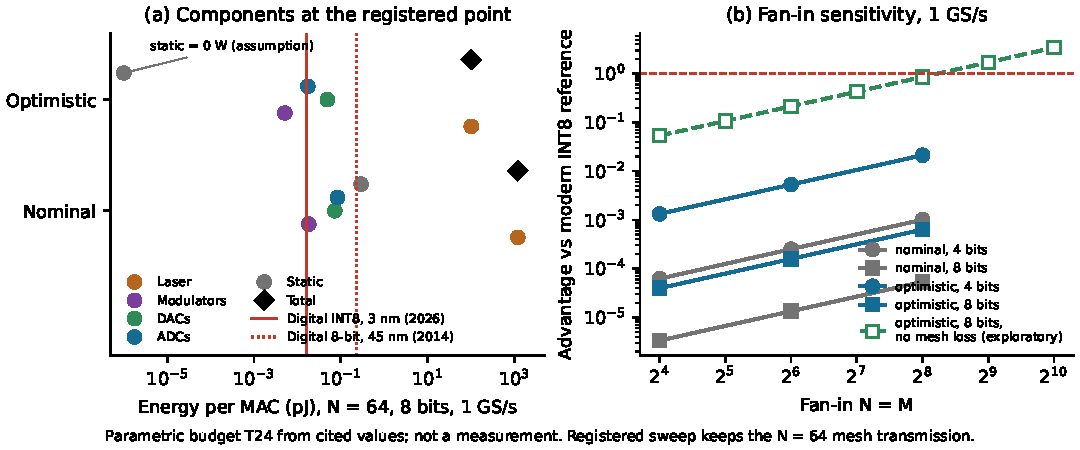
\includegraphics[width=\linewidth]{figures/fig_t24_energy.pdf}
\caption{T24 (parametric budget, cited values). (a) Energy per MAC by component at the registered point for the nominal and optimistic sets, with the two digital references. (b) Advantage factor versus fan-in; the registered sweep keeps the $N=64$ mesh transmission, and the dashed curve is an exploratory optimistic case without mesh loss.}
\label{fig:t24}
\end{figure}


\subsection{T26: state of the art and the waveguide-loss hypothesis}

\emph{Question.} Against which verified results must the project's waveguide hypothesis and its crossing argument be judged? A separate search agent followed a frozen strategy; 31 records were included and all identifiers were checked against Crossref or arXiv. The two values that decide the registered rules were re-read in the primary full text.

\textbf{Propagation loss.} The lowest verified loss we found for a fs-written single-mode guide in fused silica at 1550\,nm is $0.06\pm0.02$\dBcm, by cut-back over 13 to 2.5\,cm \cite{Ackermann2025}; 0.07\dBcm is reported by Tan et al.\ \cite{Tan2022} and, at 920\,nm, by Skryabin et al.\ \cite{Skryabin2024}. The project's hypothesis H1 (total loss $\le0.3$\dBcm for its trench guide at 1550\,nm, threshold taken from a tubular guide \cite{Bukharin2015}) is therefore a feasibility test, not a state-of-the-art claim. It was amended before any measurement (mode HE$_{11}$, one three-zone rule, one leakage reference) and complemented by H1-SOTA with threshold 0.06\dBcm. No verified depressed-cladding loss at 1550\,nm was found; a 2025 telecom-band study in SK1310 glass \cite{Zhou2025} could not be read and must be checked before any priority statement.

\textbf{Crossings and networks.} The only verified per-crossing figure is an upper bound: at most 0.01\,dB per intersection at 80$^\circ$ in fused silica at 1550\,nm, with crosstalk below a $-40$\,dB floor \cite{Djogo2026}. Crossing-free three-dimensional Fourier-transform circuits \cite{Crespi2016}, large programmable meshes \cite{Pentangelo2024,Kondratyev2024} and a multilayer three-dimensional photonic neural network in glass \cite{Cao2026} already exist.


\section{Central claim and decisive test}

The registered rules give the following picture. Energy advantage (H-A) fails its test, robustly against modern digital hardware. With the lowest verified crossing loss, the planar crossings of a butterfly cost about 0.11\,dB on the worst path at $N=16$, less than one S-bend of 0.4--0.5\,dB reported by the same source \cite{Djogo2026}; by rule I1, recomputed for the better layout, the crossing argument survives only for $N\ge64$, at the edge of the rule, and it has a 2016 precedent. In-situ calibration (H-C) is supported in the model but is established practice. With the advice of the local decision model (consulted with recorded provenance), we chose one central claim:

\begin{quote}
\textbf{Central claim.} For fs-laser-written waveguide meshes in glass with the component values found, (a) three-dimensional connectivity can save at most one layer of a universal mesh of two-mode elements; (b) at $N=64$ and 8 bits the converters and modulators alone cost 1.4--4.5 times a 3\,nm INT8 macro per MAC, independently of the optical core, and with the single published interferometer-stage loss a dense passive layer needs 0.10\,nJ per MAC; (c) crossings alone do not decide a three-dimensional advantage, because at the only verified crossing loss they cost less than the transitions a three-dimensional route needs.
\end{quote}

This is a delimitation supported by numerical models and verified literature, not a measurement. Its own decisive measurements are the loss per cascaded interferometer stage in fs-written silica (at most 0.13\,dB would reverse the comparison with the 2014 reference) and the loss of series crossings and of one three-dimensional transition. The first wording of this claim was corrected after an adversarial review (Supplementary records T20 and T30). The next \emph{physical} test of the waveguide programme, a separate claim, is registered but not run: a blind cut-back of HE$_{11}$ at 1550\,nm on trench guides with $t=12$\,\textmu m (H1, feasibility) and $t=16$\,\textmu m (H1-SOTA). For the second geometry the exact vector solver predicts an ideal leakage floor of 0.0020\dBcm (0.0440\dBcm at 12\,\textmu m), so the test would measure scattering and absorption against the state of the art rather than leakage.


\section{Discussion}

\paragraph{What holds.} The depth bound (at most one layer saved), the crossing counts and the converter floor of the energy budget do not depend on the mesh choices: the comparison with modern digital hardware is lost even for a lossless optical core. In-situ calibration absorbs splitter errors of 0.02\,rad in the model, for $N\le8$ and ideal access to the transfer matrix.

\paragraph{What is refuted.} The energy-efficiency motivation for a dense passive mesh in glass, under the stated architecture and present components, and the novelty of three-dimensional multilayer fs-written networks and of crossing-free three-dimensional Fourier circuits.

\paragraph{What cannot be concluded.} Nothing here is measured. The energy test is specific to a mesh realization of a dense layer; architectures based on fan-out and photoelectric multiplication, free space or wavelength multiplexing need their own registered tests. The crossing value is an upper bound at one angle. The calibration model omits crosstalk, drift and measurement noise. The waveguide loss of the project's trench geometry is unknown until samples exist.

\paragraph{Process and review.} Only two of the four registered tests had falsifiable criteria (energy and calibration); the depth/crossing study and the literature review were verification gates. The energy test failed, one run crashed and was repeated under a dated amendment, and two candidate novelty claims were withdrawn. An independent adversarial review recomputed the budget (relative difference $10^{-16}$), found a better planar layout, sharpened the depth bound and showed that the first wording of the energy and crossing claims overstated their evidence; the claims above are the corrected ones. All tests were designed and run by AI agents under the author's direction with self-recorded timestamps; an external timestamp and external human review are still missing.


\section*{Reproducibility, data and code}
All code, protocols, commitment records, audits, raw results and negative results are in the public repository (branch \texttt{main} after the merge of 13 October 2026). Each test is reproduced on one CPU thread with \texttt{python -B experimentos/<test>/run\_<test>.py}; the claims table is regenerated with \texttt{tools/build\_claims\_ledger.py}. The repository has no license yet (owner decision pending); until one is chosen, reuse needs the owner's permission.

\section*{Use of AI assistance}
Language models assisted with code, analysis and drafting: Claude (Anthropic) wrote the kill-test code, ran the tests, gathered and identifier-checked the literature and drafted this text; Codex (OpenAI) wrote much of the earlier solver code; the local model JEV was consulted for routing decisions. The author directed the project and is responsible for the content. AI agents are not authors, and their mutual agreement is not treated as independent verification.

\section*{Author contributions}
F.\,A.\,de\,L.: conception, direction, decisions. No experimental partner has contributed yet.

\bibliographystyle{unsrt}
\begin{thebibliography}{99}

\bibitem{Kondratyev2024} I.~V.~Kondratyev \emph{et al.}, ``Large-scale error-tolerant programmable interferometer fabricated by femtosecond laser writing,'' \emph{Photonics Res.} \textbf{12}(3), A28 (2024). doi:10.1364/PRJ.504588
\bibitem{Pentangelo2024} C.~Pentangelo \emph{et al.}, ``High-fidelity and polarization-insensitive universal photonic processors fabricated by femtosecond laser writing,'' \emph{Nanophotonics} \textbf{13}(12), 2259--2270 (2024). doi:10.1515/nanoph-2023-0636
\bibitem{Cao2026} Cao \emph{et al.}, ``Programmable three-dimensional photonic neural network chip,'' \emph{Nat. Commun.} \textbf{17}, 5476 (2026). doi:10.1038/s41467-026-72316-9
\bibitem{Clements2016} W.~R.~Clements \emph{et al.}, ``Optimal design for universal multiport interferometers,'' \emph{Optica} \textbf{3}(12), 1460 (2016). doi:10.1364/OPTICA.3.001460
\bibitem{Hamerly2019} R.~Hamerly, L.~Bernstein, A.~Sludds, M.~Solja\v{c}i\'c, D.~Englund, ``Large-scale optical neural networks based on photoelectric multiplication,'' \emph{Phys. Rev. X} \textbf{9}, 021032 (2019). doi:10.1103/PhysRevX.9.021032
\bibitem{McMahon2023} P.~L.~McMahon, ``The physics of optical computing,'' \emph{Nat. Rev. Phys.} \textbf{5}, 717--734 (2023). doi:10.1038/s42254-023-00645-5
\bibitem{Horowitz2014} M.~Horowitz, ``Computing's energy problem (and what we can do about it),'' \emph{ISSCC Dig. Tech. Papers}, 10--14 (2014). doi:10.1109/ISSCC.2014.6757323
\bibitem{Ceccarelli2020} F.~Ceccarelli \emph{et al.}, ``Low power reconfigurability and reduced crosstalk in integrated photonic circuits fabricated by femtosecond laser micromachining,'' \emph{Laser Photonics Rev.} \textbf{14}, 2000024 (2020). doi:10.1002/lpor.202000024
\bibitem{Ackermann2025} Ackermann \emph{et al.}, ``High-speed femtosecond UV laser writing of low-loss waveguides in fused silica,'' \emph{Opt. Lett.} \textbf{50}(8), 2506 (2025). doi:10.1364/OL.557978
\bibitem{Tan2022} D.~Tan, X.~Sun, Q.~Li, J.~Qiu, ``Effectively writing low propagation and bend loss waveguides in the silica glass by using a femtosecond laser,'' \emph{Opt. Lett.} \textbf{47}, 4766 (2022). doi:10.1364/OL.470670
\bibitem{Skryabin2024} N.~Skryabin \emph{et al.}, ``Femtosecond-laser-written low-loss multiscan waveguides in fused silica,'' \emph{Phys. Rev. Appl.} \textbf{22}, 064079 (2024). doi:10.1103/PhysRevApplied.22.064079
\bibitem{Bukharin2015} M.~A.~Bukharin, D.~V.~Khudyakov, S.~K.~Vartapetov, ``Heat accumulation regime of femtosecond laser writing in fused silica and Nd:phosphate glass,'' \emph{Appl. Phys. A} \textbf{119}, 397--403 (2015). doi:10.1007/s00339-015-8990-x
\bibitem{Zhou2025} Zhou \emph{et al.}, ``Femtosecond laser writing of telecom-band depressed-cladding waveguides and mode modulation in SK1310 glass,'' \emph{Opt. Mater.} \textbf{159}, 116651 (2025). doi:10.1016/j.optmat.2025.116651
\bibitem{Djogo2026} G.~Djogo, A.~Rahimnouri, P.~R.~Herman, ``Laser structured optical interposer for ultra-dense surface coupling of multicore fibers to silicon photonic chip,'' \emph{J. Lightwave Technol.} \textbf{44}, 7978--7986 (2026). doi:10.1109/JLT.2026.3720907; arXiv:2512.01972
\bibitem{Crespi2016} A.~Crespi \emph{et al.}, ``Suppression law of quantum states in a 3D photonic fast Fourier transform chip,'' \emph{Nat. Commun.} \textbf{7}, 10469 (2016). doi:10.1038/ncomms10469

\end{thebibliography}

\end{document}
